\documentclass{article}
\usepackage[margin=2cm]{geometry}
\usepackage{tabularx}
\usepackage{booktabs}
\usepackage{multirow}
\usepackage{enumitem}
\usepackage{url}
\usepackage{graphicx}
\usepackage{caption}
\usepackage{wrapfig}
\usepackage{setspace}
\usepackage{xcolor}
\usepackage{amsmath}
\usepackage{svg}
\usepackage{hyperref} % Required for hyperlinks
\usepackage{multicol} % this package is used to divide the document into multiple columns

\makeatletter
\renewcommand{\maketitle}{\bgroup\setlength{\parindent}{0pt}
\begin{center} % Center the title
  \Large\@title
  \newline
  \footnotesize\@author
\end{center}
\begin{flushright}
  \@date
\end{flushright}
\egroup}
\makeatother

% Adjust line spacing
\setstretch{0.9}

% Adjust paragraph spacing
\setlength{\parskip}{0pt}

\begin{document}

\title{Impact of Liquidity Pool Size on Trading Volume in BTC-ETH Pools}
\author{
  Team \#111 \\
   \scriptsize Matias Vizcaino (avizcaino3) | Walter Jack Simmons (wsimmons35) | MingShen Wang (mwang709) | Vítor de Matos Castilho (vcastilho3)
}
\date{09 July 2023}
\maketitle

\noindent
% {\setlength{\tabcolsep}{4pt} % Reduce column spacing


\section*{\textbf{Problem Statement and Objective}}

Decentralized Finance (DeFi), hosting about 48.78 billion USD in total value (as of April 23, 2023\cite{defillama}), relies heavily on liquidity pools in decentralized exchanges like Uniswap for efficient crypto trading. These pools, using an automated market maker model, earn from trading fees, participation rewards, and interest, distributed among liquidity providers based on their pool share\cite{defi-characterisation-2023,impermanentloss2023,yield_farming_protocols}.

This study primarily \textbf{aims to examine the influence of pool size on trading volume, specifically in BTC-ETH liquidity pools in exchanges like Uniswap}. It hypothesizes a direct correlation between pool size and trading volume, supported by existing studies\cite{defi-characterisation-2023,risks_returns_uniswap}. This understanding could optimize liquidity provision, enhance DeFi market efficiency, and benefit stakeholders. For instance, liquidity providers could improve fee returns and risk management, traders could refine strategies, and DeFi platforms could develop more effective liquidity pools\cite{makarov2021cryptocurrencies,defi2023uniswap}.

\section*{\textbf{Uniswap Liquidity Pools: An Overview}}

Various DeFi platforms cater to different needs. Uniswap, a popular choice, provides a user-friendly interface and a broad spectrum of token pairs. Other platforms like Curve Finance and Balancer offer low-slippage trades and customizable pools, respectively\cite{yield_farming_protocols}.

Uniswap, a decentralized exchange (DEX) on Ethereum, supports trading of Ethereum-native and wrapped non-native assets. It uses a Constant Product Market Maker (CPMM) model in which liquidity providers deposit two tokens, keeping a constant product of reserves\cite{defipaper2023, risksreturns2023,defi2023uniswap}.

Uniswap v3 introduced the concept of "virtual" versus "real" reserves, where virtual reserves behave as if all liquidity is concentrated at the current price range [uniswapv3math2023]. The unique mechanism allows more efficient capital usage and offers liquidity providers the ability to customize their price exposure. Precise calculations of position holdings and pool's parameters are possible through the equations provided by the Uniswap v3 liquidity math paper [uniswapv3math2023,defi2023uniswap].[Uniswap V3's liquidity pools and the constant product market maker (CPMM) model are at the heart of the study of BTC-ETH pools. Research conducted in this area provides key insights and methodologies for predicting trading volume based on various activities within these pools \cite{defi2023uniswap}. A detailed understanding of decentralized finance (DeFi) and how it differs from traditional financial structures is crucial in order to fully comprehend the mechanics of automated market makers (AMMs) and the operation of liquidity pools \cite{makarov2021cryptocurrencies}]

The CPMM formula is given by:

\[x \cdot y = k \quad \text{and} \quad price = \frac{y}{x}\]

Here, \(x\) and \(y\) denote the quantities of Token X and Y in the pool, and \(k\) is the constant product\cite{makarov2021cryptocurrencies,defi2023uniswap}.

Uniswap operates without a central authority, ensuring privacy, fund control, and a diverse range of tokens\cite{defi2023uniswap}. Centralized exchanges (CEX), though offering faster transaction speeds and better customer support, may pose security risks as they hold user funds\cite{makarov2021cryptocurrencies}. Liquidity pools in DEXs enable direct interaction with smart contracts, ensuring continuous liquidity but exposing liquidity providers to impermanent loss risks\cite{impermanentloss2023, risksreturns2023}. Prices are influenced by trade size, market conditions, supply-demand dynamics, and external price changes\cite{defi-characterisation-2023,risks_returns_uniswap,defi2023uniswap}.

\pagebreak
\section*{\textbf{Analytical Methodology and Achievements}}

A thorough analysis of the interconnectedness between Uniswap v3 pools and a systematic selection of subsets of pools for analysis is required. This will be done over different time periods, using similar methodologies as found in recent studies \cite{defi-characterisation-2023}. The relationship between liquidity, trading volume, and price stability in pools will be examined, along with an investigation of how liquidity pool size impacts trading volume.

\begin{table}[htbp]
  \centering
  \small
  \begin{tabularx}{\linewidth}{|>{\raggedright\arraybackslash}X|}
  \hline
  \textbf{Feature Engineering:} Our models' predictive power was enhanced by creating new features from existing data\cite{defi2023uniswap}. This process effectively captured crucial information about liquidity pool dynamics, spillover effects, and price divergences. \\
  \hline
  \textbf{Modelling and Optimization:} Through the application of Ordinary Least Squares (OLS) regression, we examined the relationship between liquidity pool size and trading volume, which offered profound insights into their interplay\cite{defi2023uniswap}. Model performance was assessed using metrics such as R-squared, while we optimized feature selection, corrected multicollinearity, and explored alternative functional forms for improved model accuracy and interpretability\cite{defi2023uniswap}. \\
  \hline
  \textbf{Innovations:} Building on the reference paper, we implemented the underlying code in Python, thus creating a robust data model to explore interactions between two liquidity pools more effectively\cite{defi2023uniswap}. Furthermore, we developed a mathematical language to facilitate the data engineering aspects of the data model\cite{defi2023uniswap}. \\
  \hline
  \end{tabularx}
  \caption{Analytical Techniques and Main Contributions}
  \label{fig:analytical-techniques}
  \end{table}
  
  Substantial accomplishments were achieved at each of our research stages, leading to a robust analysis and valuable results\cite{defi2023uniswap}.

  \begin{table}[htbp]
  \centering
  \small
  \begin{tabularx}{\linewidth}{|>{\raggedright\arraybackslash}X|}
  \hline
  \textbf{Data Collection:} We sourced data from multiple APIs (Uniswap, Binance) successfully, and associated this data with Ethereum block numbers for consistent time measurement. \\
  \hline
  \textbf{Data Preprocessing:} We maintained data consistency, addressed discrepancies from different sources, and efficiently cleaned, formatted, and handled missing values in the dataset. \\
  \hline
  \textbf{Exploratory Data Analysis (EDA):} Utilizing EDA, we generated descriptive statistics, visualizations, and correlation analyses. This approach facilitated the identification of trends, outliers, and the relationships between variables. \\
  \hline
  \textbf{Final Analysis and Conclusions:} We articulated our findings and conclusions, providing quantitatively-driven insights with the potential to enhance liquidity provision, optimize trading strategies, and improve the efficiency of DeFi marketplaces. \\
  \hline
  \textbf{Confirmation of Results:} Our results largely coincide with those in the reference paper, with minor discrepancies likely due to the techniques used and features available. Notably, we utilized fewer features and feature categories than the reference paper, which might explain the minor divergences observed in our results\cite{defi2023uniswap}. \\
  \hline
  \end{tabularx}
  \caption{Supporting Work and Confirmation of Results}
  \label{fig:approach-accomplishments}
  \end{table}


Our work provides a significant contribution by offering an open framework that allows other researchers and professionals to conduct further research in this field. This outcome not only answers our problem statement but also opens avenues for future exploration\cite{defi-characterisation-2023}.

\section*{\textbf{Challenges and Insights}}

Our main challenges were data collection and processing due to intricate engineering and the rate limits of the Etherscan free-tier API\cite{etherscan_api}. Nonetheless, we overcame these hurdles and made significant progress in understanding liquidity pool dynamics\cite{defi-characterisation-2023,impermanentloss2023,defi2023uniswap}.

We embraced two time concepts—"trading clock" and "time horizon"—which enabled us to thoroughly explore both short and long-term trends. This detailed analysis offered invaluable insights for decision-making and risk management in the DeFi ecosystem\cite{defi-characterisation-2023}.

We successfully addressed complexities in understanding entry-level liquidity pool mathematics and integrated the associated formulas into calculations.py functions. This step significantly enriched our feature derivation and bolstered our overall analysis\cite{uniswapv3math2023,impermanentloss2023}.
For instance, we tackled the complexity of tick math, which involves mapping discrete ticks to continuous prices. This step, guided by the Uniswap v3 liquidity math paper, was essential for interpreting Uniswap data and indexes [uniswapv3math2023]. In addition, we adjusted raw price ratios for token decimals to get human-readable prices, a process critical for presenting our analyses [uniswapv3math2023].

[Place this into our context: It is also important to acknowledge the economic and security risks inherent to these protocols. Economic risks such as yield dilution, conversion risk, exchange risk, counterparty risk, and liquidation risk all pose challenges to the sustainability and effectiveness of yield farming \cite{yield_farming_protocols}. Moreover, security risks, including flash loan attacks, rug pulls, reentrancy, and key exploits are also prevalent in the yield farming landscape \cite{yield_farming_protocols}]

\textbf{Key Note:}
\begin{itemize}
\item Our main focus during the development process was programming and data structure, leading to our code's modular design. Consequently, the mathematical formulas used in the feature engineering stage were not rigorously tested or based on an in-depth understanding of the underlying liquidity mathematics. There is room for improvement, and we encourage peer-review of the calculations.py module. The modular nature of our model presents a prime opportunity for further research\cite{uniswapv3math2023,defi2023uniswap}.
\item Our models, although providing useful insights, might benefit from a more detailed understanding of the underlying liquidity mathematics, as provided by the Uniswap v3 liquidity math paper [uniswapv3math2023]. We encourage rigorous testing and peer review of our calculations.py module to ensure accuracy and completeness of our results\cite{uniswapv3math2023,defi2023uniswap}.
\end{itemize}
\section*{\textbf{Dataset}}

In line with the \textit{"DeFi modeling and forecasting trading volume" (2023)} study\cite{defi-modeling-2023}, we gathered and structured trade data spanning a minimum of 6 months. Our GitHub repository provides more details and the code used to gather this information\cite{github-repo}. Our dataset incorporates information from the following sources:

\begin{table}[ht]
  \centering
  \small
  \begin{tabular}{|p{0.15\linewidth}|p{0.35\linewidth}|p{0.5\linewidth}|}
  \hline
  \textbf{Source} & \textbf{Description} & \textbf{Data} \\
  \hline
  Uniswap's The Graph API\cite{uniswap_graph_api} & This API offers transaction details, trading volumes, and block data from Uniswap v3 liquidity pools. & Includes transaction IDs, timestamps, amounts, USD equivalents, and other related data. \\
  \hline
  Etherscan API\cite{etherscan_api} & Utilized to extract corresponding transaction data from Etherscan based on transaction hashes. & Block hashes, block numbers, sender addresses, gas details, transaction hashes, and other relevant information. \\
  \hline
  Binance\cite{binance_cex_data} & Provides Centralized Exchange (CEX) data for ETHBTC trades. Data was obtained via scripts from Binance's GitHub repository. & Contains detailed data about each trade performed on the Binance platform, including trade prices, quantities, timestamps, and buyer/seller characteristics. \\
  \hline
  \end{tabular}
  \caption{Dataset Source Description}
  \label{tab:dataset-description}
  \end{table}


\section*{\textbf{Key Variables}}

\textbf{Target Variable:} The key dependent variable in our study is the trading volume of liquidity pools (amountUSD) over specific blocks. We propose several models for different time horizons to investigate how the relationships evolve over time.

\textbf{Independent Variables:} The independent variables are constructed from various features and are grouped as follows:

\begin{enumerate}[label=\arabic*. ,itemsep=0pt, topsep=0pt]
\item \textbf{Direct Pool Features (41):} These include measures such as volatility, rate, number of trades, and average trade size.
\item \textbf{CEX Spillover Effects (6):} This category includes variables like actual coin trade volume on Centralized Exchanges (CEX), which can influence liquidity pools on decentralized platforms.
\end{enumerate}

\section*{\textbf{Engineering Ecosystem}}

Data engineering and feature extraction are crucial elements for building robust predictive models. In the case of analyzing BTC-ETH trading volume on Uniswap, several aspects of data must be considered.

First, let's consider the nature of the data we are dealing with. Uniswap is a decentralized exchange that operates on an automated market-making (AMM) model, and its Version 3 (v3) utilizes a novel mechanism of concentrated liquidity pools. The structure and dynamics of these liquidity pools play a crucial role in trading volumes \cite{defi2023uniswap}. We must extract relevant data from these pools, including their sizes, trading volumes, and related metrics, for accurate analysis. Understanding DeFi's goals and mechanisms from a broad perspective is also valuable \cite{makarov2021cryptocurrencies}.

Moreover, it's important to incorporate data from different sources, considering not just the pools of interest but also neighboring pools and other prominent exchanges such as Binance. This kind of broad-spectrum data helps in capturing spillover effects, which are significant drivers of trading volume \cite{defi2023uniswap}. For example, we can study the effects of trading volume and the activities from interconnected DeFi protocols and stablecoins \cite{defi-characterisation-2023}.

Feature selection is a crucial part of the process. Stepwise regression can be an effective tool for optimizing the model and refining the set of independent variables \cite{defi2023uniswap}. We should also account for factors like network effects, economies of scale, and concentration issues that can influence liquidity provision \cite{makarov2021cryptocurrencies, defi-characterisation-2023}.

From a risk perspective, we should account for external risks to liquidity providers like arbitrage opportunities, fraudulent DEXs, regulatory risks, censorship risks, etc. \cite{impermanentloss2023}. Systemic risks from interconnected DeFi protocols and stablecoins could also impact trading activity \cite{makarov2021cryptocurrencies}. Additionally, economic risks like yield dilution, conversion risk, exchange risk, counterparty risk, and liquidation risk pose challenges and should be considered \cite{yield_farming_protocols}.

For the implementation part, we can take advantage of mathematical equations and formulations. For example, we can use equations to calculate the amounts of assets based on liquidity, price range, and the current price \cite{uniswapv3math2023}. Formulas for calculating impermanent loss and changes in holdings after a price change could also be useful in our analysis \cite{uniswapv3math2023, impermanentloss2023, risksreturns2023}.

\section*{\textbf{In-Depth: Feature Engineering}}

Feature engineering plays a crucial role in capturing the dynamics and relationships between variables in our analysis. The focus lies on engineering features that capture historical patterns of the DEX pools and spillover effects from CEX activity.

To start with, we can first define all the blocks in scope, then move to define the Reference blocks, and finally, the interval between reference blocks (which will be all the blocks in the interval).

Let's assume $B$ is the entire sequence of blocks within the scope of analysis and $K$ is the total number of blocks under study. We can represent this in the following way:

\begin{equation}
B = \{b_k\}_{k=1}^{K} \text{ where each } b_k \text{ is a block within the scope of analysis}
\end{equation}

In the construction of a time-series data model, the "Reference Block" acts as a chronological reference point. These blocks are key markers within the blockchain, identified based on Mint Operations when users provide liquidity to different pools on the decentralized exchange (DEX), such as Uniswap. The Reference Blocks are categorized into "same" and "other" pools. We position the most recent at the top and with an index of 0, so the sequence of blocks is ordered in decreasing chronological order.

\begin{equation}
R_{s} = \{b_{s}\}_{s=1}^{S} \text{ where each } b_{s} \in B \text{ and is a reference block in the "same" pool}
\end{equation}

\begin{equation}
R_{o} = \{b_{o}\}_{o=1}^{O} \text{ where each } b_{o} \in B \text{ and is a reference block in the "other" pool}
\end{equation}

Here, $S$ and $O$ are the total number of reference blocks in the "same" and "other" pools respectively.

Finally, the intervals between these reference blocks, which contain all blocks between $b_i$ and $b_j$ (inclusive of $b_i$), can be defined as the sequence of block numbers between $b_i$ and $b_j$. This can be expressed as:

\begin{equation}
I = \{b_{ij}\}_{\substack{i=0,j=i+1 \ i,j\leq N}}^N
\end{equation}

In this formula, $b_{ij}$ represents the sequence of blocks from $b_i$ to $b_{j-1}$, inclusive of $b_i$ and exclusive of $b_j$. This correctly captures the notion of an interval being all blocks "between" $b_i$ and $b_j$ in the blockchain sequence.

Block Reference Interval chains for the "same" and "other" pools' mint operations generate sequences of block numbers. These chains include the last N reference blocks and every block in between, where N signifies the number of lags or intervals analyzed for the direct features. Let $C_{s}$ and $C_{o}$ be the chains of "same" and "other" pools, which can be mathematically defined as:
\begin{equation}
C = \{b_{i}\}_{i=0}^{N} \text{ where each } b_{i} \text{ is a block} \in \{R_s, R_o\} \text{ and } b_{i} > b_{i+1} \text{ for } i \in \{0,1,...,N-1\}
\end{equation}

Time horizons, representing future periods or timeframes for predictions or analyses of target variables, are constructed by starting from the first Reference Block and increasing the block count by M until the next reference block is reached. 
[TODO -> Define M]
\begin{equation}
H_{M} = \{b_{0}+kM\}_{k=0}^{K} \text{ with } K = \min \left( K_{\text{max}}, \left\lfloor \frac{\text{distance to next reference block}}{M} \right\rfloor \right)
\end{equation}

\begin{figure}[htbp]
\begin{minipage}{0.5\textwidth}
\centering
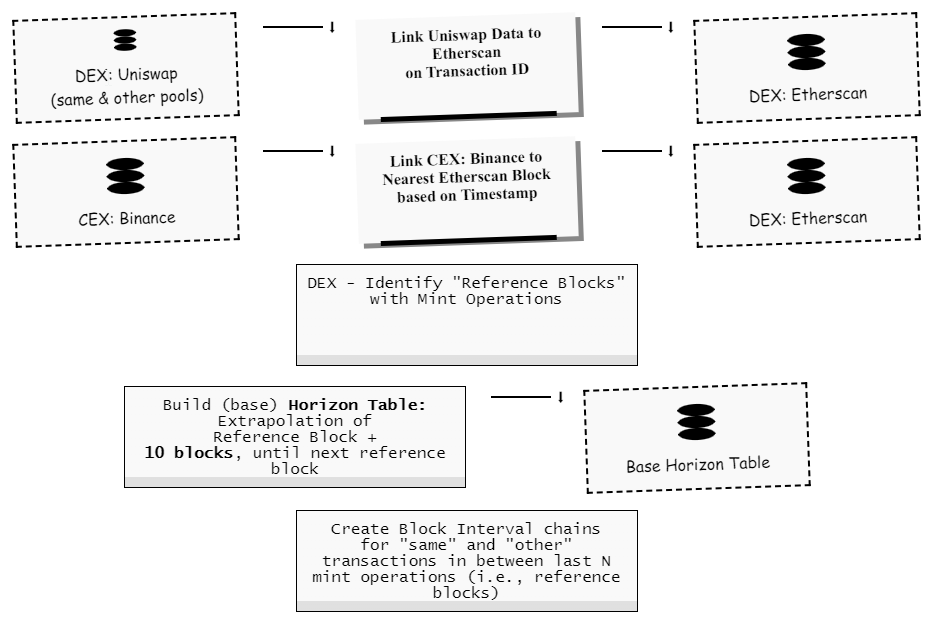
\includegraphics[width=\linewidth]{C:/Users/MatiasVizcaino/repos/6203-DataAnalyticsBusiness-Project/Other Resources/data-diagram/engineer.png}
\caption{Data Engineering}
\label{fig:data-diagram-engineer}
\end{minipage}
\begin{minipage}{0.45\textwidth}
\centering
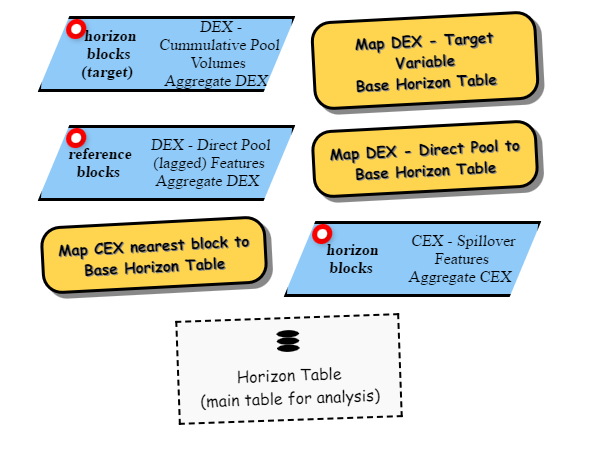
\includegraphics[width=\linewidth]{C:/Users/MatiasVizcaino/repos/6203-DataAnalyticsBusiness-Project/Other Resources/data-diagram/features.png}
\caption{Feature Engineering}
\label{fig:data-diagram-features}
\end{minipage}
\end{figure}

The Horizon Block Table captures the dynamics and relationships between the same/other/both pools by evaluating their respective target variables and features at different horizons and lags. The granularity level varies for each component within the Horizon Block Table, as illustrated in the following table:

\begin{equation}
HBT = \{ (H_{M}, F_{\text{DEX}}, F_{\text{DP}}, F_{\text{CEX}}) \} \text{ for each horizon } H_{M} 
\end{equation}

\begin{table}[htbp]
\centering
\begin{tabular}{|c|c|}
\hline
\textbf{Component} & \textbf{Granularity Level} \\
\hline
DEX target variable & Horizon block level \\
\hline
DEX direct pool features & Reference block level \\
\hline
CEX spillover features & Horizon block level \\
\hline
\end{tabular}
\caption{Granularity Level of Components in Horizon Block Table}
\label{table:granularity}
\end{table}

This granularity distinction allows for comprehensive examination of the behavior and interactions of the "same" and "other" pools at different levels within the time-series data model. The Horizon Block Table provides insights into the dynamics of the analyzed data, revealing the collaborative or competitive dynamics between the "same" and "other" pools throughout the time series.

TODO -> Table of the values we use on our project. Mention that the combination provides a rich set of models for analysis

\section*{Data Profiling Report}
This report provides an analysis of our data profiling exercise, focusing on block intervals, transaction types, reference blocks, and target variables. We aim to develop a comprehensive understanding of our dataset, paving the way for more robust model fitting and further analysis.

The data merging process between Uniswap transactions and Etherscan demonstrated a high match rate of transactions for the six-month analysis period, affirming the integrity of our dataset. Further cleaning and integrity checks were performed on each of the sources for facilitating subsequent processing.

\subsection{Block Intervals and Transactions}
The dataset encompasses block intervals ranging from 0 to 3, where block time refers to the number of blocks between reference blocks that carry out a mint operation, in both the same and other pools. A pattern of increasing block time and transaction count is observed as we transition from the most recent to preceding intervals. The maximum block time recorded is 8,497 for the 500 pool and 8,460 for the 3000 pool, both at intervals 2 and 3. The maximum row count approximates 1,115, indicating substantial data captured within these intervals.

Transaction data, classified as 'burns', 'mints', and 'swaps', reveals 'swaps' to be the prevalent transaction type across all dates and both the 500 and 3000 pools. However, the volume of each transaction type exhibits variations over time, illustrating the dynamic nature of the market. The 500 pool consistently records higher transaction volumes across all types and dates, implying a greater liquidity or popularity of the 500 pool. The number of burns and mints transactions generally balance, signifying an equilibrium between supply inflow (mints) and outflow (burns), with occasional deviations.

\subsection{Reference Blocks}
Reference blocks form a critical component in our analysis. Our dataset accommodates different numbers of reference blocks for the 500 (3,242) and 3000 (4,986) pools, with each block serving as a reference point for recording block time and transaction count. An unusual surge in mint activity recorded in July 2022 merits further investigation to uncover potential market influences or events during that period.

\subsection{Target Variables}
The target variables in our dataset comprise 'cum\_volume\_500', 'cum\_volume\_3000', and 'cum\_volume\_base' for the 500, 3000, and both reference pools, respectively. These variables encapsulate cumulative volumes across different pools and underpin our forthcoming modeling and analysis.

\subsection{Data Cleaning and Preprocessing}
Prior to the modeling phase, it was essential to address records with missing values in the independent variables. Specifically, we identified null values in the volatility (same pool) and avg-USD/rate-USD (other pool) metrics. We deployed Python utility functions customized for Pandas DataFrame to conduct the initial data cleaning and preprocessing. These tasks comprised identifying and addressing missing values, eliminating correlated columns, and aggregating data at specific intervals.

\begin{itemize}
    \item \textbf{Handling Missing Values:} [CHECK THIS SECTION] Certain columns such as 'rate-USD-iother\_01', 'avg-USD-iother\_01', 'vol\_0\_1', 'vol\_0\_2', 'vol\_0\_3' contained null values, which we replaced with zeros to render the dataset suitable for model fitting. However, a few columns like 'slother\_3', 'rate-count-iother\_23', 'wlother\_3' continued to accommodate a significant number of null values. Further decisions regarding these null values remain unindicated.
    \item \textbf{Correlated Features:} [Insert Matrix] We identified columns such as 'blsame\_2', 'blsame\_3', 'blother\_2', 'blother\_3', 'vol\_0\_1', 'vol\_0\_2' as highly correlated, leading to their removal from the dataset to prevent multicollinearity during model fitting.
    \item \textbf{Column Aggregation:} We aggregated certain columns that shared prefixes like 'rate-count-isame\_', 'rate-count-iother\_', 'binance-btc-', summing up their data in new columns appended with '03'. We subsequently dropped the original columns.
    \item \textbf{Data Loss Assessment:} We meticulously tracked the change in row count during the data cleaning process, which led to an insignificant data loss of 0.09\% observations, denoting a successful data cleaning operation with the majority of the data preserved.
\end{itemize}

\subsection{Data Preparation for Model Fitting}
We prepared three Horizon Tables (refbase, ref500, ref3000) for each mint of reference, leading to a total of 118,785 horizons. Before proceeding to fit the Ordinary Least Squares (OLS) models, we limited the horizons to a maximum of 30, which with K=10 it corresponds to about 300 blocks and $\sim$2.3 minutes (given a mean block time of 14 seconds). This step allows us to focus on the most immediate blocks, thereby reducing noise and enhancing the robustness of our modeling process.

% add new line
In conclusion, our detailed data profiling has enabled us to unearth critical insights into block intervals, transaction types, reference blocks, and target variables. Despite certain challenges such as missing values and high correlation among variables, strategic management of these issues ensures minimal data loss. This thorough comprehension of our data lays a robust foundation for the subsequent stages of our data exploration and analysis pipeline.


\section*{\textbf{In-Depth: Modelling Techniques}}

In our analysis, we will employ regression models to investigate the relationship between liquidity pool size and trading volume. Specifically, we will use an Ordinary Least Squares (OLS) regression approach.

We will develop and test OLS regression models for different target variables and horizons. Lagged variables will be incorporated into the models to predict trading volumes at different time horizons. The performance of the models will be evaluated using metrics like R-squared.

Additional modelling techniques and considerations, such as addressing autocorrelation, endogeneity, structural breaks, and multicollinearity, will be applied to enhance the accuracy and interpretability of the models.


We have commenced the development of a framework for our prediction models and have constructed several Proof of Concept (PoC) models. For the modeling phase, we're employing an Ordinary Least Squares (OLS) regression approach to predict multiple target variables across different horizons using a set of independent lagged variables for each reference mint. This process involves iterating over the horizons, generating data subsets, fitting an OLS model for each horizon, and retrieving the R-squared value as a performance indicator. This approach allows for efficient and consistent prediction across various horizons.

\[
\text{{cum\_volume\_500}}_\text{{horizon}} = \beta_0 + \beta_1 \cdot \widetilde{01}X + \beta_2 \cdot \widetilde{12}X + \beta_3 \cdot \widetilde{23}X + \ldots + \epsilon
\]

In this formula, \(\beta_0\), \(\beta_1\), \(\beta_2\), \(\beta_3\), etc., represent the coefficients associated with each spot lagged variable, while \(\epsilon\) denotes the error term or residual.

\begin{wrapfigure}[16]{l}{0.35\textwidth}
\vspace{0pt} % Adjust the vertical spacing as needed
\centering
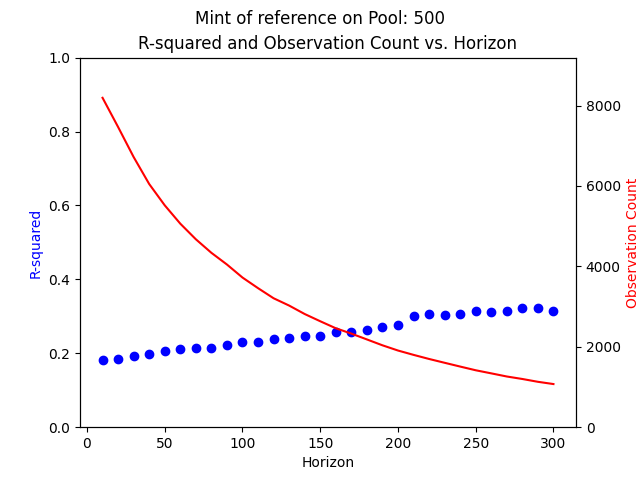
\includegraphics[width=\linewidth]{C:/Users/MatiasVizcaino/repos/6203-DataAnalyticsBusiness-Project/Other Resources/R2Horizon.png}
\caption{R2 best fit horizon}
\label{fig:R2-horizon}
\end{wrapfigure}

Observations indicate that around the horizon 20 (200 blocks, approximately 13 minutes), the R2 value ceases to increase significantly. Preliminary analysis of the relevant model (at horizon 20) reveals that the OLS regression model explains approximately 27.6\% of the variation in the dependent variable cum\_volume\_3000\_ref500. The significant variables, such as rate-count-isame\_01, rate-count-isame\_12, rate-count-isame\_23, and wlother\_3, have a considerable impact on the dependent variable. However, the potential collinearity among the independent variables could affect the interpretation of individual coefficients, suggesting a need for further analysis.

Model selection will be based on the optimal combination of features for each horizon. As we refine the feature and model development, considerations like autocorrelation, endogeneity, structural breaks, or multicollinearity will be addressed. These will be managed through additional sensitivity analyses, cross-validations, and the application of appropriate statistical techniques to diagnose and mitigate any complexities.


\section*{\textbf{Model Optimisation and Selection}}

Once the initial models are developed, we will evaluate their performance and optimize them for better accuracy and predictive power. Model optimization may involve refining the feature selection, reducing multicollinearity, and exploring alternative functional forms or transformations of variables.

Model selection will be based on the optimal combination of features, horizons, and target variables that provide accurate predictions and meaningful insights.

\section*{\textbf{Analysis and Discussion}}

In the final stages of our analysis, we will conduct an in-depth examination of the results and draw conclusions based on the findings. We will analyze the relationships between liquidity pool size and trading volume in BTC-ETH pools, considering other factors such as spillover effects and price divergences.

We will discuss the implications of our findings for liquidity provision, DeFi market efficiency, and various stakeholders. The quantitative-driven insights from our analysis can help optimize liquidity provision, refine trading strategies, and improve the effectiveness of liquidity pools in the DeFi ecosystem.


[Overall, this work aims to provide a comprehensive understanding of the dynamics of liquidity pools in the context of Uniswap V3. By leveraging the insights and methodologies from recent research \cite{defi2023uniswap, makarov2021cryptocurrencies, defi-characterisation-2023, impermanentloss2023, yield_farming_protocols, risksreturns2023, uniswapv3math2023}, this study seeks to enrich the discourse on the impact of liquidity pool size on BTC-ETH trading volume]

\section*{Going Forward}

To summarize, the learnings from this project, particularly regarding data engineering and feature generation, are substantial. This largely unexplored field of financial technology presents vast opportunities for fresh findings and contributions to the existing body of knowledge. Our initial results are promising, and we're eager to delve into the forthcoming phases of our project, emphasizing model optimization and refining our analysis and conclusions.

Our future steps in the modeling phase include:

\begin{itemize}
\item Dataset Splitting: Partitioning the dataset into training and test sets, performing model metrics analysis, and interpretation.
\item Analysis Scope: Examining both Pool 500 and Pool 3000, with a focus on target variables related to volume on the same pool as the reference mint, the other pool, or both.
\item Experimentation: Identifying the optimal combinations of features, horizons, and target variables for accurate predictions.
\item Feature Selection: Using techniques like step-wise or Principal Component Analysis to reduce feature complexity, limit overfitting, and improve interpretability.
\end{itemize}

Our planned experiments include testing different lag lengths, incorporating quadratic features or interaction terms, and accounting for structural breaks, such as the Terra-Luna collapse (May 2022) and the Merge (Sep 2022).

We aspire here or on further work to drive a comprehensive analysis and quantitative discussion on:

\begin{enumerate}[itemsep=0pt, topsep=0pt]
\item The relationship between liquidity pool size and trading volume in BTC-ETH liquidity pools.
\item The influence of the liquidity pool size on the slippage in BTC-ETH trading pairs, considering CEX spillover effects.
\item Impact of BTC-ETH price volatility on trading volume relative to liquidity pool size, focusing on price divergence.
\item Specific periods/events that significantly affect the relationship between BTC-ETH liquidity pool size and trading volume.
\end{enumerate}



\section*{\textbf{Future Extensions}}
Future extension:

Future extensions may include price divergences in BTC-ETH exchanges and pools, as arbitrage opportunities may also drive activity.

\begin{enumerate}[label=\arabic*. ,itemsep=0pt, topsep=0pt]
\item Direct pool features (2): total value locked (TVL)
\item Network spillover effects (8): trade flow imbalance.
\item Price divergences between the 500 and 3000 pools (2).
\end{enumerate}

[A key concept to understand in this analysis is the notion of impermanent loss. The impermanent loss function for Uniswap v2 liquidity providers is a notable concept to be included in the discussion \cite{impermanentloss2023}. The role of yield farming protocols, their classification, and their sources of yield are also significant considerations in this analysis \cite{yield_farming_protocols}]

\section*{Appendix}

From the transaction data, we created 8,228 reference blocks that correspond to each mint operation. These blocks were then used to engineer features to calculate metrics for the same pool and other pools. These features capture data about liquidity pools and calculate metrics such as volatility, traded volume rate, trades count, and average volume. To expand the analysis, we have also included lagged features for the previous three mint operations. Table \ref{table:chains} serves as our block reference table.
\begin{table}[htbp]
  \centering
  \small
  \begin{tabularx}{\linewidth}{|X|r|l|l|}
    \hline
    \textbf{pool} & \textbf{reference\_blockNumber} & \textbf{same\_blockNumberChain} & \textbf{other\_blockNumberChain} \\
    \hline
    500 & 14498564 & [14498564, nan, nan, nan] & [14498564, nan, nan, nan] \\
    500 & 14498699 & [14498699, 14498564, nan, nan] & [14498699, nan, nan, nan] \\
    500 & 14499597 & [14499597, 14498699, 14498564, nan] & [14499597, 14499560, 14499457, 14499198] \\
    500 & 14499836 & [14499836, 14499597, 14498699, 14498564] & [14499836, 14499560, 14499457, 14499198] \\
    500 & 14500355 & [14500355, 14499836, 14499597, 14498699] & [14500355, 14500043, 14499560, 14499457] \\
    ... & ... & ... & ... \\
    3000 & 15648981 & [15648981, 15648330, 15648305, 15648187] & [15648981, 15648887, 15648536, 15646933] \\
    3000 & 15649246 & [15649246, 15648981, 15648330, 15648305] & [15649246, 15649243, 15648887, 15648536] \\
    3000 & 15649545 & [15649545, 15649246, 15648981, 15648330] & [15649545, 15649522, 15649347, 15649269] \\
    3000 & 15649565 & [15649565, 15649545, 15649246, 15648981] & [15649565, 15649522, 15649347, 15649269] \\
    3000 & 15649578 & [15649578, 15649565, 15649545, 15649246] & [15649578, 15649522, 15649347, 15649269] \\
    \hline
  \end{tabularx}
  \caption{Block Interval Chains}
  \label{table:chains}
\end{table}

Finally, we've constructed a base table \ref{tab:horizon} with the \texttt{start\_blockNumber} of each horizon and the \texttt{reference\_blockNumber}, defined by mint operations in the block. This base table is joined with the mint aggregated transaction data to generate our target variables and independent variables that are lagged.

\begin{table}[htbp]
  \centering
  \small
  \begin{tabular}{cccccc}
    \hline
    \textbf{horizon\_blockNumber} & \textbf{min\_flag} & \textbf{reference\_blockNumber} & \textbf{horizon\_label} & \textbf{cum\_volume\_500} \\
    \hline
    108757 & 0 & 15552674 & 9 & 423,485.34 \\
    108758 & 0 & 15552674 & 10 & 423,485.34 \\
    108759 & 1 & 15552772 & 1 & 328,338.73 \\
    108760 & 0 & 15552772 & 2 & 406,084.78 \\
    108761 & 0 & 15552772 & 3 & 536,640.71 \\
    ... & ... & ... & ... & ... \\
    109047 & 0 & 15555464 & 12 & 122,730.73 \\
    109048 & 0 & 15555464 & 13 & 123,650.59 \\

    \hline
  \end{tabular}
  \caption{Example: Horizon Table (reference mint on pool=3000)}
  \label{tab:horizon}
\end{table}

% \textbf{Adapting Mathematical Formulas:} We adapted the formulas from the Uniswap v3 liquidity math paper for calculating impermanent loss and changes in holdings after a price change. This adaptation helped us demonstrate P&L calculations and provided a deeper understanding of Uniswap's dynamic [uniswapv3math2023].



\bibliographystyle{alpha} % You could use plain, unsrt, alpha, abbrv etc. 
\bibliography{references}
% \usepackage[style=verbose-note, url=true]{biblatex}
%
\end{document}